% UQ QOL/EQUS Poster format
% Forked from: https://www.overleaf.com/project/618cc965bcbc81513871601f
% Credit: Ali Furkan Kalay
% See: https://github.com/alfurka/gemini-uq
% Forked from
% https://rev.cs.uchicago.edu/k4rtik/gemini-uccs
% which is forked from
% https://github.com/anishathalye/gemini


\documentclass[final]{beamer}

% ====================
% Packages
% ====================
\usepackage[T1]{fontenc}
\usepackage{lmodern}
\usepackage[orientation=portrait,size=a0,scale=0.95]{beamerposter} % Current dimensions A0, put in your poster dimensions
\usetheme{gemini}
\usecolortheme{uchicago}
\usepackage{graphicx}
\usepackage{caption}
\usepackage{booktabs}
\usepackage{tikz}
\usepackage{pgfplots}
\pgfplotsset{compat=1.17}
\newcommand{\blu}{\color{blue}}
\usepackage{DejaVuSans}

% ====================
% Colors (dark blue theme)
% ====================
\definecolor{PosterBlue}{RGB}{16,44,92}
\definecolor{PosterBlueLight}{RGB}{230,238,252}
\definecolor{PosterBlueMid}{RGB}{43,78,140}
\setbeamercolor{palette primary}{fg=white,bg=PosterBlue}
\setbeamercolor{headline}{fg=white,bg=PosterBlue}
\setbeamercolor{footline}{fg=white,bg=PosterBlue}
\setbeamercolor{title separator}{fg=PosterBlue,bg=PosterBlue}
\setbeamercolor{block title}{fg=white,bg=PosterBlue}
\setbeamercolor{block body}{fg=black,bg=white}
\setbeamercolor{alertblock title}{fg=white,bg=PosterBlueMid}
\setbeamercolor{alertblock body}{fg=black,bg=PosterBlueLight}
\newcommand{\blocktopspace}{\vspace{0.45em}}
%%%%%%%%%%%%%%%%%%%%%%%%%%%%%%%%%%%%%%%%%%%%%%%%%%%%%%%%%%%%%%%%%%%%%%%%%%%%%%
% Column environment setup
%%%%%%%%%%%%%%%%%%%%%%%%%%%%%%%%%%%%%%%%%%%%%%%%%%%%%%%%%%%%%%%%%%%%%%%%%%%%%%
% If you have N columns, choose \sepwidth and \colwidth such that
% (N+1)*\sepwidth + N*\colwidth = \paperwidth
% Follow structure to create difference column environments. 
\newlength{\sepwidthA} % Seperation distance between comulumns type A
\newlength{\colwidthA} % collumn width type A
\setlength{\sepwidthA}{0.25\paperwidth}
\setlength{\colwidthA}{0.5\paperwidth}

\newcommand{\separatorcolumnA}{\begin{column}{\sepwidthA}\end{column}}

% Second column environment. 
\newlength{\sepwidthB}
\newlength{\colwidthB}
\setlength{\sepwidthB}{0.0666\paperwidth}
\setlength{\colwidthB}{0.4\paperwidth}

\newcommand{\separatorcolumnB}{\begin{column}{\sepwidthB}\end{column}}

% You can also use these column commands to create columns inside columns and for creating new column formatting. 
% You can also have non even columns by creating more column environments or specifying the width when beginning a column environment. 
%%%%%%%%%%%%%%%%%%%%%%%%%%%%%%%%%%%%%%%%%%%%%%%%%%%%%%%%%%%%%%%%%%%%%%%%%%%%%%
% Title
%%%%%%%%%%%%%%%%%%%%%%%%%%%%%%%%%%%%%%%%%%%%%%%%%%%%%%%%%%%%%%%%%%%%%%%%%%%%%%

\title{\Huge{DEMONSTRACE VYUŽITÍ PROSTŘEDKŮ ROS 2 NA PODVOZKU\\WAVE ROVER S RASPBERRY PI, KAMEROU A LIDAREM}}
\author{\textbf{Filip Botlo}}
\institute[shortinst]{VUT v Brne, Fakulta informačných technológií, UITS}

%%%%%%%%%%%%%%%%%%%%%%%%%%%%%%%%%%%%%%%%%%%%%%%%%%%%%%%%%%%%%%%%%%%%%%%%%%%%%%
% Poster footer
%%%%%%%%%%%%%%%%%%%%%%%%%%%%%%%%%%%%%%%%%%%%%%%%%%%%%%%%%%%%%%%%%%%%%%%%%%%%%%

\footercontent{
\href{mailto:xbotlo01@stud.fit.vut.cz}{xbotlo01@stud.fit.vut.cz}
  \hfill
  Bakalárska práca -- 2026
  \hfill
  Vedúci: doc. Ing. Vladimír Janoušek, Ph.D.}
% (can be left out to remove footer)  

\begin{document}
%%%%%%%%%%%%%%%%%%%%%%%%%%%%%%%%%%%%%%%%%%%%%%%%%%%%%%%%%%%%%%%%%%%%%%%%%%%%%%
% Header logos removed for clean academic style.

% ====================
% Body
% ====================

\begin{frame}[t]
\begin{columns}[t]
%%%%%%%%%%%%%%%%%%%%%%%%%%%%%%%%%%%%%%%%%%%
%Section 2 column 1
%%%%%%%%%%%%%%%%%%%%%%%%%%%%%%%%%%%%%%%%%%%
\separatorcolumnB

    \begin{column}[T]{\colwidthB}
    \footnotesize

        \begin{block}{Cieľ práce}
            \blocktopspace
            Cieľom bolo navrhnúť a implementovať modulárny riadiaci softvér pre mobilnú platformu
            \textbf{Wave Rover} s využitím \textbf{ROS 2} na \textbf{Raspberry Pi 5}.

            \vspace{0.4em}
            Riešenie pokrýva:
            \begin{itemize}
                \item manuálne riadenie a motorový uzol (\texttt{DriveNode}),
                \item autonómne režimy (wander, jednoduchá bodová navigácia),
                \item spracovanie dát zo senzorov (LiDAR, IMU, kamera),
                \item webové rozhranie, runtime prepínanie režimov a monitoring.
            \end{itemize}
        \end{block}

        \begin{block}{Platforma a architektúra}
            \blocktopspace
            \begin{figure}
                \centering
                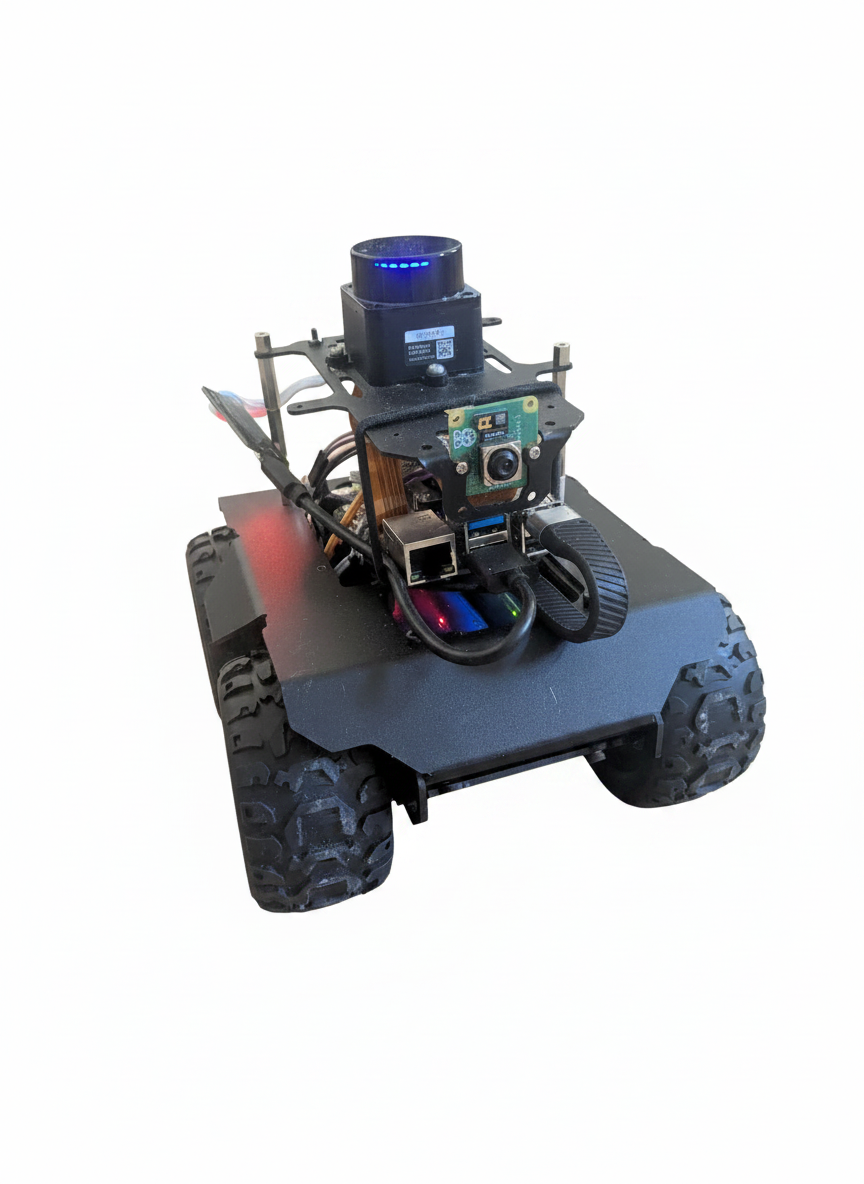
\includegraphics[width=0.950\textwidth,clip,trim=0 220 0 120]{Figures/rover.png}
            \end{figure}
            \vspace{0.2em}
            Architektúra je rozdelená do troch vrstiev:
            \begin{itemize}
                \item \textbf{Senzorická}: LiDAR LD19, IMU (MPU-6050), kamera,
                \item \textbf{Riadiaca}: motorový uzol, korekcie jazdy, autonómne režimy,
                \item \textbf{Integračná}: launch súbory, prepínanie režimov, web UI.
            \end{itemize}
        \end{block}

    \begin{block}{Hlavný prínos}
        \blocktopspace
        Výsledkom je funkčný, modulárny ROS 2 systém, ktorý prepája manuálne ovládanie,
        autonómne správanie, spracovanie senzorov a webové rozhranie do jednej prakticky
        použiteľnej platformy pre experimenty v mobilnej robotike.
    \end{block}

    \begin{block}{Kľúčové technológie}
    \blocktopspace
    \textbf{ROS 2 Jazzy}, \textbf{Raspberry Pi 5}, \textbf{Wave Rover}, \textbf{LiDAR LD19},
    \textbf{MPU-6050}, \textbf{OpenCV}, \textbf{Gazebo Sim}, \textbf{RViz2},
    \textbf{WebRTC}, \textbf{rosbridge/roslibjs}.
    \end{block}
        
\end{column}
\separatorcolumnB
%%%%%%%%%%%%%%%%%%%%%%%%%%%%%%%%%%%%%%%%%%%
%Section 2 column 2
%%%%%%%%%%%%%%%%%%%%%%%%%%%%%%%%%%%%%%%%%%%
\begin{column}[T]{\colwidthB}
\scriptsize

    \begin{block}{Prepojenie bežiacich uzlov}
        \blocktopspace
        \begin{figure}
            \centering
            
\includegraphics[width=0.80\linewidth]{Figures/runtime_rqt.png}
        \end{figure}
    \end{block}

    \begin{block}{Debug detekcie objektu}
        \blocktopspace
        \begin{figure}
            \centering
            
\includegraphics[width=0.80\linewidth]{Figures/pomaranc.png}
        \end{figure}
    \end{block}

    \begin{block}{Porovnanie odchýlky jazdy}
        \blocktopspace
        \begin{figure}
            \centering
            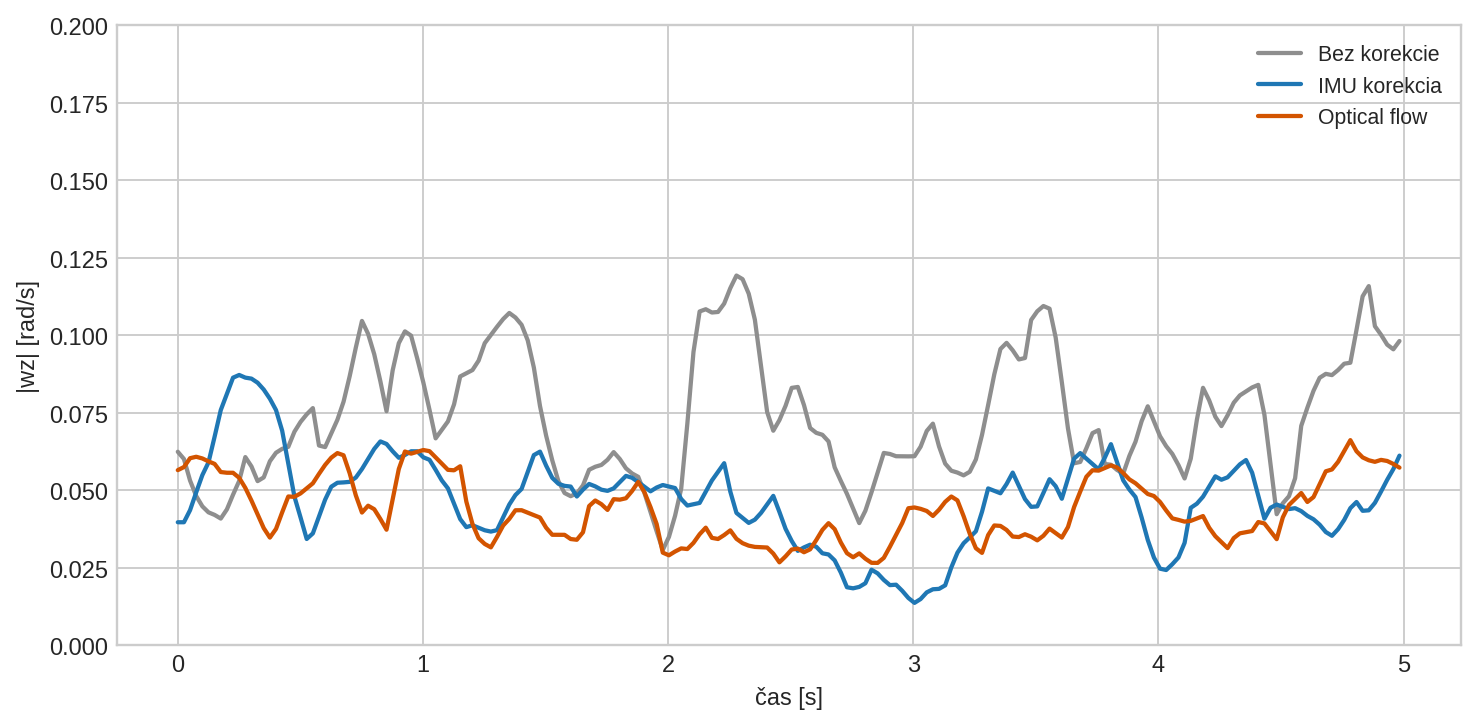
\includegraphics[width=0.80\linewidth]{Figures/odchylka_porovnanie_3_rezimy_5s.png}
        \end{figure}
    \end{block}

    \begin{block}{Výsledky testovania}
    \blocktopspace
    Testovanie prebiehalo v interiéri na fyzickom robote a čiastočne v simulácii.
        \begin{table}
            \centering
                \begin{tabular}{@{}p{0.29\textwidth}p{0.61\textwidth}@{}}
                \toprule
                \textbf{Oblasť} & \textbf{Pozorovanie} \\
                \midrule
                Manuálne riadenie & Stabilné, plynulé prepínanie medzi vstupmi. \\
                Wander režim & Spoľahlivo reaguje na prekážky v bežných podmienkach. \\
                IMU korekcia smeru & Stabilná aj pri slabšom osvetlení, vhodná pre prevádzku. \\
                Optický tok & Presný pri dobrej textúre/scéne, citlivý na svetlo. \\
                Sledovanie lopty & Funkčné po doladení HSV, citlivé na svetelné podmienky. \\
                \bottomrule
            \end{tabular}
        \end{table}
    \end{block}

    \begin{block}{Limity a ďalší vývoj}
        \blocktopspace
        \begin{itemize}
            \item \textbf{Limity}: chýbajúce enkodéry, drift IMU, citlivosť vizuálnych metód na osvetlenie.
            \item \textbf{Ďalšie kroky}: presnejšia odometria, robustnejšia fúzia senzorov a pokročilejšie metódy spracovania obrazu.
        \end{itemize}
    \end{block}

\end{column}
\separatorcolumnB
\end{columns}
\end{frame}
\end{document}
